\documentclass[11pt,onecolumn]{article}
%\documentclass[10pt,twocolumn]{article}

\usepackage[utf8x]{inputenc}
\usepackage{balance}
\usepackage{multirow}
\usepackage{chngpage}
\usepackage{booktabs}
\usepackage{url}
\usepackage{color}
\usepackage{needspace}
\usepackage{verbatim}
\usepackage{tikz}
\usetikzlibrary{arrows}
\usetikzlibrary{matrix}
\usetikzlibrary{shapes}
\usetikzlibrary{scopes}

\newcommand{\code}[1]{\texttt{#1}}
\newcommand{\todo}[1]{\textcolor{red}{#1}}

\title{Implementation Details of Dynamic Information Flow Security Type Systems}

\author{Eric~Hennigan \hspace{12pt} Christoph~Kerschbaumer \\ Stefan~Brunthaler \hspace{12pt} Michael~Franz\\
\\
Department of Information and Computer Science\\
University of California, Irvine, CA 92717\\
\\
Tech. Report 11-03\footnote{This material is based upon work supported in part by the National Science Foundation under Grant No. CNS-0905684.}
}


\begin{document}

% got the TR number on July 7
\date{July 21, 2011}

\maketitle

\begin{abstract}
% state the problem
Existing dynamically typed languages, such as JavaScript, do not offer strong security guarantees even though they handle sensitive information.
% say why it's an interesting problem
Augmenting the runtime environment with a security type system capable of tracking implicit information flows requires extensive modifications.
% say what your solution achieves
We analyze two options that support a security type system orthogonal to the existing type system.
% say what follows from your solution
After considering implementation issues such as primitive values, interned objects, and garbage collection, we conclude that security typing is best accomplished via additional tag bits representing the security types.
\end{abstract}

\thispagestyle{empty}
\newpage
\setcounter{page}{1}

\section{Introduction}

An extensive amount of research in information flow security focuses on enforcement through sound type systems~\cite{1159651}.
Because information flow security can be phrased as a static type analysis~\cite{volpano1996sound}, current research strongly focuses on adding security to statically typed languages, such as Java~\cite{myers2001jif}.
We believe that dynamically typed languages should receive an equivalent, if not greater, amount of attention towards security.

JavaScript~\cite{ecma}, for example, powers Web~2.0, supporting electronic commerce, social networking, and web applications.
These applications allow people to share with friends, manage digital profiles, purchase goods and services, and pay bills electronically.
As a site becomes popular and hosts more information, such as client contact data and credit card numbers, it also becomes an enticing target for fraud and information theft.

For example, the website Mint.com~\cite{mint.com} allows users to manage all their financial accounts, through a single online interface.
To provide this service, Mint.com requires users to input their login credentials for banks and other financial institutions.
Although Mint.com provides a ``read-only'' service for monitoring and budgeting, the very storage of financial credentials presents a lucrative target for identity thieves.

To help websites prevent accidental information leakage, we design a dynamic information flow security type system that adds information flow protection to JavaScript, a dynamically typed language.
We introduce a security type system that is orthogonal to the built-in JavaScript type system and which dynamically enforces information flow security.
Practicality of this framework rests on the modification of a popular and full featured implementation of JavaScript.
In this paper, we report our experience of implementing information flow in SpiderMonkey, the JavaScript interpreter powering Mozilla's Firefox web browser.

We consider two possible implementations of security types (see Section~\ref{sec:implementation}): extending of the tagged pointer representation and introducing a security wrapper object.
We examine how each option affects the labeling of primitive values and interned objects, and how the labeling mechanism will impact memory requirements and the garbage collector (see Section~\ref{sec:analysis}).
We corroborate this analysis with a report on our experience during implementation (see Section~\ref{sec:experience}).
Finally, we discuss how our work compares with that of others (see Section~\ref{sec:related-work}), and finish with a recommendation that an extension of the tagged pointer representation meets the requirements of a dynamic information flow security type system and has the least implementation effort (see Section~\ref{sec:conclusion}).

\section{Implementing Runtime Security Types}\label{sec:implementation}

Before discussing the details of the two possible implementations of dynamic security types, we first give a review of the existing dynamic type system that SpiderMonkey employs.

\subsection{Existing Type System}

Many implementations of dynamically typed languages follow a common approach of using a tagged union to represent each possible primitive or object reference type~\cite{gudeman1993representing}.
In SpiderMonkey, this union takes the form of a 64-bit word.
As illustrated in Figure~\ref{fig:base-encoding}, the lower 47 bits of the word contain the value payload, while the upper 17 bits encode the type.
This type can be one of \texttt{double}, \texttt{int32}, \texttt{undefined}, \texttt{boolean}, \texttt{magic}, \texttt{string}, \texttt{null}, or \texttt{object}.
The SpiderMonkey virtual machine (VM) uses the \texttt{magic} type for internal purposes, such as tracking holes in dynamically sized arrays and distinguishing an exception thrown by a generator vs. one thrown by a program or runtime error.

\begin{figure}[h]
\centering
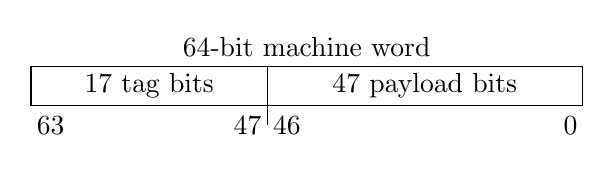
\begin{tikzpicture}[scale=.5]
 %\node at (7, 3) {\texttt{jsval} layout};
 \draw[anchor=center] (7,1.5) node {64-bit machine word};
 \draw (0,0) -- (0,1) -- (14,1) -- (14,0) -- cycle;
 \draw[anchor=center] (3,.5) node {17 tag bits};
 \draw (6,-.5) -- (6,1);
 \draw[anchor=center] (10,.5) node {47 payload bits};
 \node at (.5,-.5) {63};
 \node at (5.5, -.5) {47};
 \node at (6.5, -.5) {46};
 \node at (13.7, -.5) {0};
\end{tikzpicture}
% from jsval.h
%#define JSVAL_PAYLOAD_MASK           0x0    0    0    0    7     FFF FFF FFF FF LL
% => payload is                                             3  +   4*12 = 51
%#define JSVAL_TAG_MASK               0xF    F    F    F    8     00000000000LL
%                                       1111 1111 1111 1111 1000
\begin{tabular}{cr | l }
  tag bits & value & type \\
\hline
  \texttt{0..0000} & 0x00 & \texttt{double} \\
  \texttt{0..0001} & 0x01 & \texttt{int32} \\
  \texttt{0..0010} & 0x02 & \texttt{undefined} \\
  \texttt{0..0011} & 0x03 & \texttt{boolean} \\
  \texttt{0..0100} & 0x04 & \texttt{magic} \\
  \texttt{0..0101} & 0x05 & \texttt{string} \\
  \texttt{0..0110} & 0x06 & \texttt{null} \\
  \texttt{0..0111} & 0x07 & \texttt{object} \\
\end{tabular}
 \caption{The dynamic type encoding mechanism used by the SpiderMonkey VM.}
 \label{fig:base-encoding}
\end{figure}

Some values in JavaScript do not fit into the 47 bits of payload.
The SpiderMonkey VM deals with these types by storing the value in a managed memory region and a pointer to that value in the payload.
For example, the VM interns \texttt{string}s and \texttt{double}s in specifically optimized memory arenas, while it places \texttt{object}s in a garbage collected heap.
We refer to values which fit directly in the payload as \emph{primitives}.

\subsection{Fat Value Technique}\label{sec:fat-values}

We can achieve dynamic information flow security by attaching, onto each runtime value, additional bits which encode a pointer, handle, or taint value representing the security type.
We term this technique the \emph{fat value} approach, and extend the existing core representation with an additional 64-bit word to hold the security type.
As shown in Figure~\ref{fig:fat-encoding}, each core value within the interpreter then becomes 128-bits, and contains both the originally encoded value and its security tag.

\begin{figure}[h]
\centering
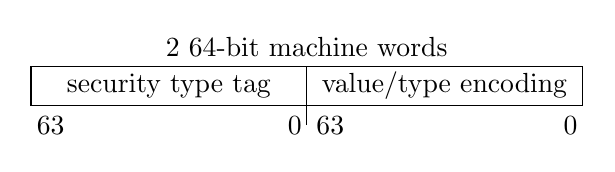
\begin{tikzpicture}[scale=.5]
 \draw[anchor=center] (7,1.5) node {2 64-bit machine words};
 \draw (0,0) -- (0,1) -- (14,1) -- (14,0) -- cycle;
 \draw[anchor=center] (3.5,.5) node {security type tag};
 \draw (7,-.5) -- (7,1);
 \draw[anchor=center] (10.5,.5) node {value/type encoding};
 \node at (.5,-.5) {63};
 \node at (6.7,-.5) {0};
 \node at (7.6,-.5) {63};
 \node at (13.7,-.5) {0};
\end{tikzpicture}
 \caption{Fat value encoding scheme.}
 \label{fig:fat-encoding}
\end{figure}

The fat value technique requires modifying the core representation of all values within the VM.
Performing this modification on such a low-level aspect of a VM is not a trivial undertaking.
The SpiderMonkey implementation contains a large number of places where manual type inspection occurs, so that an operation may be correctly dispatched.
To ensure that the change in representation does not adversely affect program execution, we need to inspect each of these dispatch sites for security implications.
Additionally, doubling the size of the core datatype also doubles the memory requirements of any running program: the VM allocates twice as much space for the same number of core values.

%\needspace{4\baselineskip}
%Extending the tagged pointer representation has the following effects:
%\begin{description}
% \item[Pro] Core values also store their security label, providing easy access during all operations.
% \item[Con] Doubles the memory requirements of all values.
% \item[Con] Affects the type dispatch code dispersed in many places throughout the VM.
%\end{description}

\subsection{Security Wrapper Technique}\label{sec:cloaks}

The goal of attaching a security label to each value can be achieved through another mechanism.
By extending objects with an internal field that stores the security label, we are able to label objects.
We can implement a security labeling mechanism on primitive values by wrapping them inside another object.
We shall refer to a wrapper which carries a security label for the purpose of enforcing information flow security as a \emph{cloak}.
Figure~\ref{fig:security-wrapper} provides a visualization of the cloak mechanism.

\begin{figure}[h]
 \centering
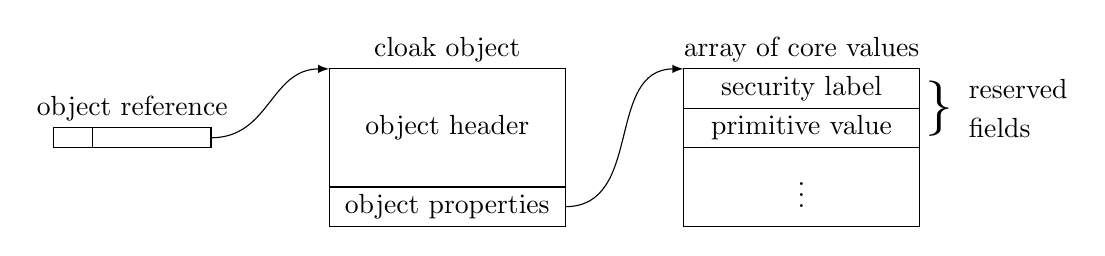
\begin{tikzpicture}[scale=.5]
 \draw[anchor=center] (3,4.5) node {cloak object};
 \draw (0,0) rectangle (6,4);
 %\draw[anchor=center] (3,4) node {$\vdots$};
 %\draw[anchor=center] (3,4.5) node {\todo{object fields ... prototype .. parent}};
 \draw[anchor=center] (3,2.5) node {object header};
 \draw (0,1) -- (6,1);
 \draw[anchor=center] (3,.5) node {object properties};
 \draw[-latex] (6,.5) .. controls (8,.5) and (7,4) .. (9,4);

 \draw[anchor=center] (-5,3) node {object reference};
 \draw (-7,2.5) rectangle (-3,2);
 \draw (-6,2.5) -- (-6,2);
 \draw[-latex] (-3,2.25) .. controls (-1.5,2.25) and (-1.5,4) .. (0,4);

 \node at (12,4.5) {array of core values};
 \draw (9,0) rectangle (15,4);
 \node at (12,3.5) {security label};
 \draw (9,3) -- (15,3);
 \node at (12,2.5) {primitive value};
 \draw (9,2) -- (15,2);
 \node at (12,1) {\vdots};

 \draw[anchor=west] (16,3.5) node {reserved};
 \draw[anchor=west] (16,2.5) node {fields};
 \node[scale=2] at (15.5,3) {\}};

\end{tikzpicture}
 \caption{Security wrapper scheme.}
 \label{fig:security-wrapper}
\end{figure}

Internally, SpiderMonkey already supports wrapper classes for a number of other security features.
For example, within Firefox, the garbage collector compartmentalizes objects based on their web origin and employs cross-compartment wrappers to enforce the cross origin access policy\cite{wagner2011}.
Given this information, we might expect fewer modifications to be made to the underlying VM, as this change only requires the introduction of a new wrapper class.

However, implementing wrapper classes is not exactly trivial, even with the help of an existing framework.
Under no circumstances should the presence (or absence) of a security wrapper ever become evident to a JavaScript program, otherwise attacker provided code could exploit the difference in behavior.
We make an exception to this guideline for policy violations, which have the side effect of halting the VM.
The wrapper must remain visible to the VM, however, so that it can enforce information flow security.

Meeting this restriction is not presently possible using the existing security wrapper framework.
The primary goals of the existing wrapper classes are to provide reference monitor security at the level of objects.
As a result, the design of the existing framework for creating wrapper classes does not sufficiently take into account the behavioral differences between objects and primitives.
Consequently, the existing framework poses an imperfect fit for implementing information flow security, because it does not guarantee perfect transparency (from the perspective of a JavaScript program) when used to wrap primitives.

%\needspace{4\baselineskip}
%Extending the system with a security wrapper has the following effects:
%\begin{description}
% \item[Pro] We do not have to modify the core representation of all values.
% \item[Pro] The VM can allocate memory to a wrapper only when a value needs to be explicitly labeled.
% \item[Con] We introduce a new class of \texttt{object} and take great care to ensure its complete transparency from the perspective of a JavaScript program.
% \item[Con] The label of a primitive value is held by the wrapper object and is not part of the value itself, so it is not directly accessible during operations.
%\end{description}

\section{Impacts on the Virtual Machine}\label{sec:analysis}

Now that we have introduced two viable techniques for implementing information flow security, we analyze how each performs when labeling primitives, how each handles interned objects, and what impacts each has on the garbage collector.

\subsection{Labeling Primitives}\label{sec:primitives}

The existing core datatype in SpiderMonkey enables the value and type tag to coexist in the same memory structure.
Although the tagged pointer encoding is an implementation detail, this decision has had side effects which have leaked into the JavaScript specification.
For example, SpiderMonkey's original 32-bit implementation used 1 bit for the integer type tag, and 31 bits for integer values.
This design forced the language specification~\cite{ecma} to provide a coercion of any integer which cannot be represented by 31-bits to the \texttt{double} type.

The tagged pointer technique has the benefit of allowing the VM to perform operations on primitives quickly and directly.
Unfortunately, many common operators, such as \texttt{+}, behave differently depending on the types of the arguments.
Not only does the VM first inspect the type of the core values involved before dispatching the operation, but it also unpacks the payload of the arguments from their encoding.
This runtime type inspection logic disperses itself across the VM implementation.

Using the fat value approach requires modifying the core value representation, extending it with additional bits to hold the security type.
This modification impacts the mechanisms used to encode and decode primitive values, as well as the type inspection routines.
Additionally, we must manually audit each site at which the VM performs runtime type inspection for potential security issues.

Alternatively, using the cloak approach requires the creation of a wrapper object for each labeled primitive.
Although the cloak easily holds both the core value representation of the primitive as well as the security type, the presence of a cloak object impacts the runtime type inspection logic.
Where before the VM would see a primitive, it now sees a cloak object.
The cloak needs to assist the VM in correctly dispatching any type sensitive operations.
This extra layer of indirection severely impacts the performance of the very operations for which primitives are optimized.

%Introducing cloaks to the VM creates further difficulties in places where the VM uses primitive values as a convenient holder for simple data items.
%For example, SpiderMonkey stores the length field of an Array as a primitive integer.
% no, i checked the source code. it's stored as a private field.
%However, information flow security demands that the length field be tagged with a security type recording how its value has been influenced.
%Thus, cloaking the length field complicates the Array implementation.

Mozilla has designed SpiderMonkey as an embeddable interpreter.
Systems external to the JavaScript engine, such as the GUI and DOM frameworks of the Firefox browser, implement their own object classes which they hand into the SpiderMonkey VM.
The fields and properties on these objects are technically external to SpiderMonkey, but are created through an API that allows SpiderMonkey to manipulate them through standard JavaScript operations (e.g., property lookups and assignments).
Cloaking such values can cause an error in the framework implementation.
For example, these frameworks make type sensitive assumptions about these properties, and fail when a cloak object appears where the framework expects a raw primitive.

Not only do we have to prohibit cloaks from escaping the VM and becoming visible to framework code, but we must also implement cloaks such that they remain completely transparent to the JavaScript programmer.
For example, even though we implement cloaks as a native \texttt{object} within the VM, we cannot allow a JavaScript program to set a property on a cloaked primitive.
Nor do we wish to add an additional special case in the VM implementation to handle cloak objects at each place type inspection occurs.

Satisfying these constraints is difficult.
For example, let us examine how the \code{typeof} operator might work.
To maintain transparency at the JavaScript level, the cloak object reports the type of the value it cloaks, and not the type of itself.
A cloaked integer returns ``number'' rather than ``object''.
However, simply dispatching the \code{typeof} operator to the wrapped value causes the cloak to lie about its own type.
Should the VM use this information in a type dispatch, it could then pass the core value encoding the cloak, which takes the form of an object reference, to native functions expecting primitive values.

When we compare the fat value approach to the cloak approach, we see an interesting semantic difference as well:
In the fat value approach, we attach the security type to the primitive value or object reference, as part of the tagged pointer encoding.
In the cloak approach, objects receive an internal field to store the security label while we label primitives with an extra layer of indirection.
%Conceptually, it is possible that a single primitive becomes wrapped by two different cloaks, whereas the fat value approach maintains only a single label for each tagged primitive. -- No, it isn't. each cloak holds its own copy of the primitive it wraps

%\needspace{4\baselineskip}
%To summarize:
%\begin{description}
% \item[Fat Values:]~\\
%  \begin{description}
%  %\item[Pro] Extending the tagged pointer representation attaches the label to the primitive, providing direct access.
%  \item[Con] The VM places extra tag bits on all core values, whether necessary for security or not.
%  \item[Con] The extra security tag affects the type dispatch code distributed throughout the VM.
%  \end{description}
% \item[Cloaks:]~\\
%  \begin{description}
%  \item[Pro] Cloaking is only necessary when labeling a primitive.
%  \item[Con] Cloak objects move operations on labeled primitives into a slow path.
%  \item[Con] Cloak objects cannot be used universally on all primitives without changing the implementation of builtin objects to support overloading of certain operators.
%  \item[Con] The presence of a cloak cannot produce observable effects, even to embedding environments.
%  \end{description}
%\end{description}

% I haven’t fully explored the difference between having a labeled reference vs having a labeled object, but I think the difference is analogous to having an Access Control Listing by columns vs Object Capabilities by rows, as discussed in Capability Myths Demolished.
% At this point I am in favor of the fat value approach, because I’m liking the reference semantics, and the transparency with which primitives can be labeled. I’m also willing to accept the cost of having fatter values.

\subsection{Interned Objects}\label{sec:interned-objects}

The SpiderMonkey VM employs optimizations pioneered by earlier dynamically typed languages, such as Lisp and Scheme.
To achieve better runtime performance and reduce memory footprint, the VM interns the \code{string} type.
Although this optimization enables much faster string comparison, the fact that two different string references may point at the same interned string object affects issues of identity.
Within an information flow framework, we need a way to record the security context of creation as well as the contents of a new object.

Using the cloak approach, we store the security label of a string in the string object itself.
As a side effect of interning strings, references to strings containing the same contents point to the same object.
Because the object stores the security label, it now becomes possible to create a function that returns a string carrying an incorrect label (see Figure~\ref{fig:interned-string}).
Although two strings may contain the same contents, we need to ensure that the attached labels can distinguish the code paths and security contexts on which each object depends.

\begin{figure}
\begin{verbatim}
function foo(x) {
  var a = "String"    // interned with the same security label
                      // as the code for function foo

  if (x) {            // the label of "a" needs to reflect
    var b = "String"  // a dependence on "x", but should not
    return b          // affect the label attached to "a"
  }

  return a
}
\end{verbatim}
 \caption{A function returning the value ``\code{String}'' which can carry one of two different security labels depending on runtime control flow.}
 \label{fig:interned-string}
\end{figure}

One solution to this dilemma is to automatically upgrade the label attached to the interned string.
However, as each occurrence of the string will upgrade the attached security label, even when such occurrences are completely independent, this causes unnecessary upgrades.
With each successive use of the interned string, the upgraded label propagates throughout the system, becoming a source of label creep.
This strategy propagates a false dependence when completely separate and non-interfering programs use the same string object purely as a side effect of referencing the same interned string.

Another possible solution is to generate a cloak around the string reference.
We prefer this strategy over the previous one, because it allows two different references to contain different security labels, allowing the system to distinguish the security contexts on which the references depend.
However, this strategy complicates the labeling guidelines:
If the VM cloaks primitives and directly labels objects, introducing logic that handles interned objects represents a special case.
Once we remove this special case, we arrive at a semantics where references to interned objects carry the security label, rather than objects themselves.

Interestingly, the fat value approach already provides such semantics.
No additional provisions are made for the special case of interned objects, as all object references also carry a security label, by virtue of extending the tagged pointer representation.

%\needspace{4\baselineskip}
%To summarize:
%\begin{description}
% \item[Fat Values:]~\\
% \begin{description}
%  \item[Pro] provide labeled reference semantics.
% \end{description}
% \item[Cloaks:]~\\
% \begin{description}
%  \item[Con] provide labeled object semantics.
% \end{description}
%\end{description}

\subsection{Garbage Collection}\label{sec:garbage-collection}

In both the fat value and cloak approaches, any security data structures, such as a runtime lattice of security labels, add to the memory requirements of the system.
Because both approaches share this memory overhead, we do not consider it as part of the following analysis.

The cloak approach creates an entire object for each value that requires labeling.
Creating these wrappers can drastically lower the performance of the overall system, and stress the garbage collection.
As labels propagate throughout a running program, we find that cloaked values become more common than not.
By creating an object for each of these labeled values, we force the garbage collector to spend much more time in both the mark and sweep phases.
Because primitives are both common and meant to be performant, we should also try to avoid expensive memory allocation calls required when creating a cloak object to label such primitives.

The fat value approach avoids these problems with the garbage collector by extending the representation of primitives and object references with additional bits to hold a security label.
However, this extension doubles the overall memory requirements of the system.
Both values placed on the operand stack and property fields within an object increase by the amount of space necessary for the attached label.
However, the memory overhead required by the security labels is far less than the additional storage required when creating a cloak object.

%\needspace{4\baselineskip}
%To summarize:
%\begin{description}.
% \item[Fat Values:]~\\
% \begin{description}
%  \item[Con] Adding security labels to the tagged pointer representation doubles the memory requirements for all values.
% \end{description}
% \item[Cloaks:]~\\
% \begin{description}
%  \item[Con] The presence of cloak objects stresses the garbage collector by introducing a larger reference graph and more object allocations.
%  \item[Con] Each primitive that needs labeling incurs an object allocation.
% \end{description}
%\end{description}

\section{Experience}\label{sec:experience}

To assess the accuracy of our analysis we implemented information flow security in Mozilla's JavaScript engine, SpiderMonkey.
Although the prior analysis covering both the cloak and fat value techniques has been informed by our experience, we can only provide a detailed report on the difficulties encountered when using the security wrapper technique due to implementation effort.
Our implementation uses cloak objects (with the layout shown in Figure~\ref{fig:security-wrapper}) and does not extend the builtin \texttt{object} layout to include a security label (for reasons discussed in Section~\ref{sec:interned-objects}).

\subsection{Interaction with External Systems}
Our implementation cloaks property fields on objects when they are modified.
The cloak holds a label representing the execution context under which the modification took place.
As mentioned in Section~\ref{sec:primitives}, the GUI and DOM frameworks of the Firefox browser implement their own classes of \texttt{object}.
These frameworks then hand these custom objects into the VM for processing, and to allowing JavaScript code contained on a webpage to update these data structures.
Because of our conservative approach, the properties in these objects quickly became cloaked.

We discovered, by visiting sites the first ten sites in Alexa's Top Sites in the United States\cite{alexa}, that these frameworks performed assertions on the type of properties stored by the custom objects.
After a custom object is handed back to the framework from the VM, 
the framework exploits internal knowledge of the object's fields and layout to update internal data structures.
If the code processing these updates encounters a cloak rather than what the framework expects, a failure can occur.

To successfully view the top ten sites, we chose to whitelist these custom objects, so that our information flow framework does not wrap them in a cloak object.
We found 67 such custom objects, including \texttt{CSSStyleSheet}, \texttt{HTMLLinkElement}, \texttt{KeyboardEvent}, \texttt{XULDocument}, \texttt{Window}, and \texttt{ChromeWindow}.


\subsection{Number of Cloak Objects}
Because we chose to use the security wrapper technique, we knew that each explicitly labeled value would incur an allocation of a cloak object. 
Initially, we strove to minimize this memory overhead by implicitly labeling values wherever possible.
We developed the following guidelines for deciding when cloaking is necessary: (1) a value cannot be implicitly labeled by its position on the operand stack or (2) if some other cloak was involved the production of the value.

We attempted to implicitly label values on the operand stack.
However, we discovered that such a labeling requires complex logic, and a naive approach is not precise.
Our implementation statically instruments JavaScript programs such that, at runtime, the VM holds a stack of labels in correspondence with the block level scope of statements under execution.
Initially, we thought that this data structure would be enough to assign labels to values on the operand stack at runtime.
However, the security label present in the label stack only represents the current execution context.
Thus it only provides a lower bound of the correct label to ascribe to a value on the operand stack.

Values on the operand stack can be produced by security contexts not represented by the scope in which a statement using that value appears.
For example, the return value from a function is labeled at least as secure as the function code itself.
However, a function callee might have a higher security label than that of the caller.
The value returned by the callee can therefore have a higher security label than that of the statement consuming the value in the caller.
Because of this possibility, our implementation explicitly cloaks values before they are returned by a function.

We also attempted to cloak a value only if another cloak is present in the calculation of that value.
This guideline minimizes the creation of cloaks based on the assumption that the presence of a cloaked value implies a security label which cannot be inferred implicitly.
Both function calls and references to cloaked objects stored in the heap can make a cloak appear in part of a calculation.
In testing our implementation, we found that label creep led to a steady rise in the number of values that need to be explicitly labeled by a cloak.

As a consequence of these observations, rather than support the logic necessary to compute implicitly labeled values, our implementation of information flow conservatively labels all values by wrapping them in a cloak object after every operation.
This dramatically hurts performance, because the VM performs a label calculation for each operation, and the input labels for this calculation can only be accessed indirectly through cloaking objects.

\begin{comment}
\subsection{SpiderMonkey uses primitive fields for convenience.}
As depicted in Figure~\ref{fig:object-layout}, an object consists of a linear array of the core representation type, \texttt{jsval}.
Each object reserves some entries for internal usage such as parent and prototype fields.
The author of an \texttt{object} class has the ability to reserve fields for internal use.
These entries are not necessarily one of the types mentioned in the list of base types (see Figure~\ref{fig:base-encoding}), but must be the same width in machine words.
For example, the Array class reserves a field for storing the length of an array object.
Because this field is also accessible through the \texttt{length()} method, array objects store the field as an \texttt{int} primitive.

\begin{figure}[h]
 \centering
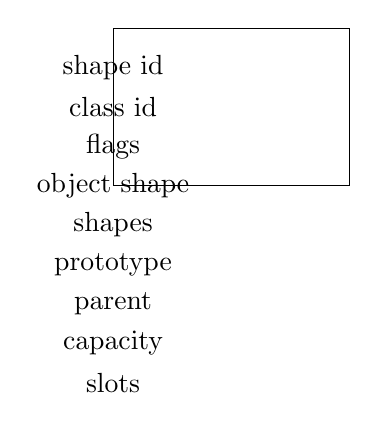
\begin{tikzpicture}[scale=.5]
 \draw (0,0) rectangle (6,-4);
 \draw[anchor=center] (0,-1) node {shape id};
 \draw[anchor=center] (0,-2) node {class id};
 \draw[anchor=center] (0,-3) node {flags};
 \draw[anchor=center] (0,-4) node {object shape};
 \draw[anchor=center] (0,-5) node {shapes};
 \draw[anchor=center] (0,-6) node {prototype};
 \draw[anchor=center] (0,-7) node {parent};f
 \draw[anchor=center] (0,-8) node {capacity};
 \draw[anchor=center] (0,-9) node {slots};
\end{tikzpicture}
 \label{fig:object-layout}
 \caption{Memory layout of an object in the Spidermonkey VM.}
\end{figure}

%Furthermore, encoding all such data into a core value simplifies object layout, because it allows an object to be composed of a linear array of fields.
%The SpiderMonkey authors found it convenient that data stored in these fields fit within the existing type system, and did not require a separate representation.
We discovered that object classes using reserved fields make assertions about the type stored in the field.
During implementation, we noticed (a) that some of these fields take on values computed by the interpreter, and (b) that some of these fields can be automatically updated in secure contexts and require a security label.
%The length field of an array object provides the most compelling example.
In both of these cases, the implementation of the object class using such fields needs to be modified in order to track information flows.
Without such modifications, SpiderMonkey either fails an assertion when a cloak appears where a primitive \texttt{int} is expected, as in case (a), or fails to track information flow through all variables, as in case (b).
\end{comment}

%typeof problem
%During implementation, we encountered this situation in several places (including the garbage collector).

\subsection{Testing}

Details regarding the code infrastructure which provides runtime tracking of information flows can be found in a companion report~\cite{tr1101}.

Our system also runs an abstract interpreter that verifies that data structures particular to our information flow framework never interfere with the normal operation of the JavaScript VM.
This analysis covers all possible executions paths for every method parsed.
We are able to run this verification over all of the more than 2,000 tests in the SpiderMonkey testing suite, which Mozilla uses to detect regressions for every code change.

We were not able to find any framework which provides a standard security benchmark on which to test information flow implementations.
As a result, we implemented 173 private test cases to ensure that we generate the correct labels for a reasonably sized subset of the control flow structures available in JavaScript.
Our system is correctly able to identify both explicit and implicit information flows represented in this test suite.
Although this effort does not substitute for a proof of correctness, it does give us confidence that our implementation faithfully follows the approach we have outlined.

\section{Related Work}\label{sec:related-work}

Over the past decades researchers have embraced the task of adding security enhancements to existing languages.
In this section, we show how our work fits into the field of information flow security and highlight related research which will likely bolster current efforts.
Our experience implementing dynamic information flow in SpiderMonkey keeps us optimistic that optimistic that a robust information flow framework can be achieved in real-world dynamically typed languages.

In 2007, Vogt et al.~\cite{Vogt_CrossSiteScripting_2007} modified an earlier version of SpiderMonkey to monitor the flow of sensitive information in the Mozilla web browser by using dynamic data tainting.
Their system explicitly identified data sources and sinks within the Firefox browser, and tags data at each source.
For each script, a static data flow analysis simulates the VM operations on an \emph{abstract stack}, to determine existence of information leaks.
Their framework handles control structures such as \texttt{throw} and \texttt{try} conservatively, by statically marking all variables within that function as tainted.

In 2010, Russo et al.~\cite{1813092} provide a mechanism for tracking information flow within the Document Object Model, a browser provided API for manipulating page layout.
This work inlines dynamic information flow monitors at the time a code string evaluates.
They demonstrate that the dreaded \texttt{eval} statement can be secured enough to satisfy the termination-insensitive non-interference property.
The proposed technique prevents the DOM from being used as a covert channel.
In contrast, our work does not address information flows present within host provided objects.

Also in 2010, Jang et al.~\cite{1866339} proposed an information flow framework for JavaScript itself based on source rewriting.
Their framework invokes a rewrite function on JavaScript code and encapsulates it into a monitored closure.
Although rewriting the source can instrument policy enforcement mechanisms, their current implementation is not capable of detecting implicit information flows.
Although they give no performance numbers, we reason that these closures incur a high memory and function call overhead, something that we seek to prevent by operating at the instruction level.

%\todo{no standard benchmarks, no standard evals, no standard info flow attacks to compare against}

\section{Summary}\label{sec:summary}

Given our analysis (cf. Section~\ref{sec:analysis}), we can now achieve a high-level overview of the two techniques for introducing security types in an existing interpreter.
Each technique features design trade-offs concerning development effort, runtime costs, and security enforcement.
We discuss these trade-offs in the context of our implementation experience (cf. Section~\ref{sec:experience}) with the SpiderMonkey JavaScript interpreter.

\subsection{Impacts on Implementation}
The fat value technique extends the tagged pointer representation of the core value type of the interpreter.
By embedding the security label into the core representation, the VM has fast and convenient access to the label on each piece of data involved in a computation.
Because the VM manipulates labels in many of the underlying opcodes, access should be kept as direct as possible.

Modifying the representation of the interpreter's core datatype can affect type-dispatch operations.
We found these operations dispersed in many places within SpiderMonkey, but expect that interpreters for other languages are similarly constructed.
To be correct in implementation, the security type author must inspect each code site to see if the new representation affects the type-dispatch.
Examining the code of SpiderMonkey reveals that the type-inspection which occurs in these dispatch operations is well-factored into macros, which dramatically eases the development effort of integrating an orthogonal security type system.

By wrapping values which need a security label in an object derived from the existing object system, the cloak technique avoids the pain of changing the core dataype representation.
We initially thought this design to be a clever advantage, but several implementation details revealed interesting and unexpected costs.

First, the cloak labels primitives indirectly.
Programmers expect primitives to behave in a performant manner, the extra level of indirection caused by a security wrapper object negatively impacts programs relying on this expectation.
When the VM performs operations on labeled primitives, it encounters an additional indirection when computing the label for the resulting value.

Second, security constraints require any cloaks which label a primitive to behave as primitives (from the perspective of the JavaScript program), not as an objects.
We found accomplishing this goal much more difficult than at first expected.
Not only must the cloaks override operators such as \code{typeof}, but they must also behave correctly under a type-dispatch operation.
When operating on a cloaked primitive, the VM encounters and dispatches on the cloak object.
This dispatch automatically places the value on a slow path, in which the cloak inspects its contents and performs the operation on the wrapped primitive.
The ability of a cloak to type-dispatch on the primitive it wraps after the VM has type-dispatched on the cloak object makes cloaks a poor fit for SpiderMonkey's existing object model.

In our experience, preventing implementation details from introducing side-effects visible at the level of a JavaScript program, such as maintaining the level of transparency required to make cloaks which wrap a primitive appear as native primitives, is difficult in practice.

\medskip
\begin{adjustwidth}{-1in}{-1in}
\begin{center}
\begin{tabular}{l|l|l}
\toprule
\multicolumn{3}{c}{Impacts on Implementation} \\
\midrule
\multicolumn{1}{c}{Concern} & \multicolumn{1}{|c|}{Fat Values} & \multicolumn{1}{c}{Cloaks} \\
\midrule
Integration      & Modifies core datatype representation & Introduces new cloak object \\
Label access     & Direct & Indirect \\
VM Type-Dispatch & Manually inspect all dispatch sites & Dispatched chained after VM \\
\bottomrule
\end{tabular}
\end{center}
\end{adjustwidth}
\medskip

\subsection{Impacts on the Runtime System}

Both the cloak and fat value techniques increase the memory size of running programs.
We focus our analysis only on the memory requirements which differ between these two techniques, and ignore memory increases, such as objects representing a label hierarchy or a runtime stack of security labels, which are common to both techniques.

By extending the core representation of all values, the fat value technique increases the memory overhead by a factor of two.
This increase extends to any core values held by internally represented JavaScript classes, such as \code{Array} or \code{RegExp} objects, so object memory requirements also increase by a factor nearly two.
In contrast, the cloak approach requires a single field be added to all objects, which the VM uses for security tagging.
The memory required by this approach is a fraction of the size of objects, and impacts the runtime system in proportion to the number of objects allocated.

On first glance, this analysis indicates that the cloak technique has a lower memory overhead in cases where the program uses many more primitives than objects.
However, when a primitive requires labeling, then the VM allocates a cloak object in which to wrap the primitive value.
Because of label creep, many primitives quickly require labeling, leading to the allocation of cloak objects.
The cloak technique only uses less memory than the fat value technique in situations where few values require labeling.
In our experience, this situation does not normally arise, because the VM labels values in many common operations (such as returns from a functions and binary operations with at least one labeled argument).

Furthermore, the allocation of a cloak object for each labeled primitive negatively affects the garbage collector, because it leads to much larger heaps, slowing down SpiderMonkey's mark-and-sweep algorithm.
The fat value technique avoids most of this cost, by reducing the number of objects held within the managed heap.
However, if the security implementation places pointers to label objects in the label half of the extended core representation then a mechanism is needed which indicates when a label object is no longer required by the security system.
The garbage collector algorithm can be re-used to produce this information, because a label object is alive only when it's pointed at by a live value.

Finally, cloaking negatively impacts runtime performance more than the fat value technique, because cloaking places the label on an indirect path.
Each time the VM performs an operation, it typically labels the resulting value with the join of the labels of all arguments.
Keeping these labels directly accessible prevents an otherwise severe runtime overhead.
Additionally, JavaScript programmers expect operations on primitives to remain performant, so the extra dispatch needed to obtain the underlying primitive from a cloak negatively impacts performance in the least desirable manner.

\medskip
\begin{adjustwidth}{-2in}{-2in}
\begin{center}
\begin{tabular}{l|l|l}
\toprule
\multicolumn{3}{c}{Impacts on the Runtime System} \\
\midrule
\multicolumn{1}{c}{Concern} & \multicolumn{1}{|c|}{Fat Values} & \multicolumn{1}{c}{Cloaks} \\
\midrule
Memory Requirements & All core values double in size & Add private tag field to all objects \\
Object Allocation   & None, every core value carries a label & Only labeled primitives require a cloak object \\
Garbage Collection  & Can use GC to keep labels alive & Increases number of objects in heap \\
Runtime Speed       & All primitives stay on fast path & Labeled primitives move to slow path \\
\bottomrule
\end{tabular}
\end{center}
\end{adjustwidth}
\medskip

\subsection{Impacts on Security Semantics}

The cloak and fat value implementations reveal important differences, not only in the interaction with a host environment, but also in the supported security semantics.

JavaScript, as an embeddable language, allows the host environment to expose functionality to client programs.
Support for this feature implies JavaScript values can be exported to the host environment.
Although it may require a re-compilation of the hosts interface code, the fat value technique allows the host environment the freedom to ignore the label extension on core values.
In contrast, the cloak technique exports labeled primitives as cloak objects, leaking the security abstraction into the host environment.
Host interface code which expects a primitive value may fault when encountering a cloak object instead.
We experienced exactly this problem when implementing cloaks in Firefox's JavaScript interpreter, SpiderMonkey.

Not only is the label in a fat value optionally ignorable, but the direct attachment of a label to the core value creates a labeled value semantics.
This semantics allows the VM to treat differently separate references to the same object, avoiding the confusion of identity that might result from having interned objects.
The cloak technique, attaches a label only to objects, and provides a labeled object semantics.
Unfortunately, because the label is attached to an object, it is shared among all references to that object.
As the object is used in different contexts, the attached label monotonically escalates, becoming a source of label creep.

\medskip
\begin{adjustwidth}{-2in}{-2in}
\begin{center}
\begin{tabular}{l|l|l}
\toprule
\multicolumn{3}{c}{Impacts on Security Semantics} \\
\midrule
\multicolumn{1}{c}{Concern} & \multicolumn{1}{|c|}{Fat Values} & \multicolumn{1}{c}{Cloaks} \\
\midrule
Visibility & VM can ignore security tag bits & Cloaks must be fully transparent \\
Security   & Labeled reference & Labeled value \\
\bottomrule
\end{tabular}
\end{center}
\end{adjustwidth}
\medskip

%Extending the system with a security wrapper has the following effects:
%\begin{description}
% \item[Pro] We do not have to modify the core representation of all values.
% \item[Pro] The VM can allocate memory to a wrapper only when a value needs to be explicitly labeled.
% \item[Con] We introduce a new class of \texttt{object} and take great care to ensure its complete transparency from the perspective of a JavaScript program.
% \item[Con] The label of a primitive value is held by the wrapper object and is not part of the value itself, so it is not directly accessible during operations.
%\end{description}

%To summarize:
%\begin{description}
% \item[Fat Values:]~\\
%  \begin{description}
%  %\item[Pro] Extending the tagged pointer representation attaches the label to the primitive, providing direct access.
%  \item[Con] The VM places extra tag bits on all core values, whether necessary for security or not.
%  \item[Con] The extra security tag affects the type dispatch code distributed throughout the VM.
%  \end{description}
% \item[Cloaks:]~\\
%  \begin{description}
%  \item[Pro] Cloaking is only necessary when labeling a primitive.
%  \item[Con] Cloak objects move operations on labeled primitives into a slow path.
%  \item[Con] Cloak objects cannot be used universally on all primitives without changing the implementation of builtin objects to support overloading of certain operators.
%  \item[Con] The presence of a cloak cannot produce observable effects, even to embedding environments.
%  \end{description}
%\end{description}


%To summarize:
%\begin{description}
% \item[Fat Values:]~\\
% \begin{description}
%  \item[Pro] provide labeled reference semantics.
% \end{description}
% \item[Cloaks:]~\\
% \begin{description}
%  \item[Con] provide labeled object semantics.
% \end{description}
%\end{description}

%To summarize:
%\begin{description}.
% \item[Fat Values:]~\\
% \begin{description}
%  \item[Con] Adding security labels to the tagged pointer representation doubles the memory requirements for all values.
% \end{description}
% \item[Cloaks:]~\\
% \begin{description}
%  \item[Con] The presence of cloak objects stresses the garbage collector by introducing a larger reference graph and more object allocations.
%  \item[Con] Each primitive that needs labeling incurs an object allocation.
% \end{description}
%\end{description}

\begin{comment}
\begin{centering}
\begin{tabular}{rl|l|l}
\toprule
  &                               & Cloaks & Fat Values \\
\midrule
{\multirow{3}{2.5cm}{Implementation}}
               & Integration      & Modifes core datatype representation & Introduces new Cloak object \\
               & Label access     & Direct & Indirect \\
               & VM Type-Dispatch & Dispatched chained after VM & Manually inspect all dispatch sites \\
\midrule
{\multirow{2}{2.5cm}{Semantics}}
               & Visibility & VM can ignore security tag bits & Cloaks must be fully transparent \\
               & Security   & Labeled reference & Labeled Value \\
\midrule
{\multirow{4}{2.5cm}{System}}
               & Memory Requirements & All core values double in size & Add private tag field to all objects \\
               & Object Allocation   & None, every core value carries a label & Only labeled primitives require a cloak object \\
               & Garbage Collection  & Keep label alive & Increases number of objects in heap \\
               & Runtime Speed       & All primitives stay on fast path & Labeled primitives move to slow path \\
\bottomrule
\end{tabular}
\end{centering}
\end{comment}


\section{Conclusion}\label{sec:conclusion}

Although both the fat value and cloak approaches can assist information flow security by adding runtime security types to all values within an existing dynamically typed language, we advocate the fat value approach, because it
(1) provides a reference semantics that works with interned objects,
(2) does not stress the garbage collector with unnecessary object creation,
and (3) easily labels every primitive and object reference.
Achieving these gains comes at the cost of:
(1) changing the representation of a core data type within the VM,
(2) auditing sites where type inspection occurs to ensure compliance with the new security system,
(3) extending all stack slots and object fields by the amount needed to store the security labels (a factor of 2).
We still consider these costs worth the associated benefits, because the cloak approach:
(1) stresses the garbage collector adding runtime overhead unrelated to security enforcement,
(2) reduces performance by adding an additional layer of indirection,
(3) does not provide a conceptually uniform treatment of objects and primitives,
and (4) is more difficult to ensure transparency from the perspective of the JavaScript programmer.

We would also like to point out that optimizations meant to improve performance, such as interning \texttt{string} objects, can have an adverse affect on security.
In particular, the interned object optimization confuses the issues of object identity and equality, in order to reduce the number of allocated objects and provide quick results for the equality (string comparison) operator.
In information flow security, the fact that two immutable objects might carry the same value implies nothing about their point of origin or the security actors which have influenced the object.
We find that the labeled reference semantics provided by the fat value technique usefully allows distinguishing the security label of an object from the value of that object.
Fortunately, this semantics means that we can keep the interned object optimization, even as we implement dynamic labeling for information flow security.

Given the difficulty and work involved in our experience we wholeheartedly corroborate the statement: ``security is not a separable concern''\cite{miller2005structure}.

\section*{Acknowledgments}\label{acks}

The authors would like to extend thanks to Gregor Wagner who has reviewed the material and ensured its accuracy.

Parts of this effort have been sponsored by the National Science Foundation (NSF) under grant CNS-0905684.
The U.S. Government is authorized to reproduce and distribute reprints for Governmental purposes notwithstanding any copyright annotation thereon.
Any opinions, findings, and conclusions or recommendations expressed here are those of the authors and should not be interpreted as necessarily representing the official views, policies, or endorsements, either expressed or implied, of NSF, or any other agency of the U.S. Government.

%In my reading of information flow security, so far, I’ve yet to see anyone that is discussing these kinds of implementation details. Many papers invent some ideal (tiny) language, then performs a proof of non-interference for that language. Without a means for translating real-world languages (with prototype chains, dynamic field lookup, generators, co-routines, exceptions, continuations, etc.) into that ideal model, we haven’t made progress. Other papers tackle a subset of the real language, and claim that the approach extends to the full language; after trying to implement this stuff myself, I seriously doubt this claim. Many language features just don’t play well together, and can seriously upset some of the hidden assumptions that allow a proof of safety for the subset to be constructed.

%CCured type-safe retrofitting of legacy code, is probably related

\balance

\bibliographystyle{abbrv}
\bibliography{tr1}


\end{document}
